\documentclass{beamer}
\usepackage{xcolor}
\usepackage{listings}

\usepackage{lmodern}
\usepackage[T1]{fontenc}
\usepackage{tikz}



\usepackage{wasysym}



\usetheme[]{Antibes}

\usetikzlibrary{automata, positioning, arrows}
\usetikzlibrary{arrows.meta, chains, positioning, quotes}

\title{Operativni sistemi}
%\subtitle[]{\textit{ - Pregled nekih zanimljivih bagova -}}
\author[Diana Šantavec]{Diana Šantavec \\ \small \url{diana.santavec@gmail.com}}
\institute{Istraživačka stanica Petnica}
\titlegraphic{\includegraphics[width=2cm]{img/Petnica.png}}
\date{20.04.2023.}


\lstset{language=C,keywordstyle={\bfseries \color{blue}}}

\setbeamertemplate{footline}
{
  \leavevmode%
  \hbox{%
  \begin{beamercolorbox}[wd=.333333\paperwidth,ht=2.25ex,dp=1ex,center]{author in head/foot}%
    \usebeamerfont{author in head/foot}\insertshortauthor
  \end{beamercolorbox}%
  \begin{beamercolorbox}[wd=.333333\paperwidth,ht=2.25ex,dp=1ex,center]{title in head/foot}%
    \usebeamerfont{title in head/foot}\insertshorttitle
  \end{beamercolorbox}%
  \begin{beamercolorbox}[wd=.333333\paperwidth,ht=2.25ex,dp=1ex,right]{date in head/foot}%
    \usebeamerfont{date in head/foot}\insertshortdate{}\hspace*{2em}
    \insertframenumber{} / \inserttotalframenumber\hspace*{2ex} 
  \end{beamercolorbox}}%
  \vskip0pt%
}

\begin{document}

% Define styles for the states
\tikzset{
  state/.style={
    circle,
    draw,
    minimum size=1cm
  },
  highlighted/.style={
    circle,
    draw,
    fill=red!50,
    minimum size=1cm,
    font=\bfseries
  }
}

\tikzstyle{process} = [rectangle, draw, text width=1cm, text centered, minimum height=1cm]
\tikzstyle{arrow} = [thick,->,>=stealth]
\tikzstyle{highlight} = [fill=red!30]
\tikzstyle{time label} = [below, align=center]

\frame{\titlepage}


\begin{frame}
\frametitle{Sadržaj}
\begin{itemize}
    \item Pojam \newline
    \item Učitavanje operativnog sistema \newline
    \item Procesi \newline
    \item Planeri procesa \newline
    \item Zaštita memorije \newline
    \item Fajl sistemi
\end{itemize}
\end{frame}

\begin{frame}
    \frametitle{Ali prvo\dots}
    \centering
    \LARGE{Čemu pokazivanje na starijoj opremi?}
\end{frame}

\begin{frame}
    \frametitle{Čemu pokazivanje na starijoj opremi?}
    \begin{itemize}
        \item Jednostavnija je \newline
        \item Neke stvari su vidljive (sada su softverske) \newline
        \item Razlog su nekih "nelogicnosti" jer se održava kompatibilnost
    \end{itemize}
\end{frame}

\begin{frame}
    \frametitle{Uvod}
    \begin{center}
        \LARGE{Šta je operativni sistem?}
    \end{center}
\end{frame}


\begin{frame}
    \frametitle{Uvod}
    \begin{itemize}
        \item Program koji omogućava aplikacijama jednostavniji pristup hardveru \newline
        \item Kontroliše izvršavanje aplikacija \newline
        \item Olakšava pisanje programa visokog nivoa \newline
        \item Omogućava nezavisnost programa od hardvera \newline
    \end{itemize}
\end{frame}

\begin{frame}
    \frametitle{Istorija}
    \begin{itemize}
        \item Prvi računari su samo izvršavali dati program (ENIAC 1945) \newline
        \item batch: učita se više programa pa se izvrše \newline
        \item 1970 - 1980 višekorisnički \newline
        \item 1980 - 1990 prvi personalni (CP/M) \newline
        \item \dots
    \end{itemize}
\end{frame}

\begin{frame}
    \frametitle{Učitavanje operativnog sistema}
    \begin{center}
        \LARGE{Šta se desi kada pritisnemo dugme?}
    \end{center}
\end{frame}

\begin{frame}
    \frametitle{Učitavanje operativnog sistema}
    \begin{itemize}
        \item Prilikom pokretanja računara operativni sistem tek treba da se učita iz neke trajne memorije \newline
        \item BIOS-MBR \newline
        \item UEFI-GPT
    \end{itemize}
\end{frame}

\section*{Učitavanje operativnog sistema}
\begin{frame}
    \frametitle{Firmware}
    \begin{itemize}
        \item Kontrola niskog nivoa \newline
        \item Na nekoj memoriji unutar uređaja \newline
        \item BIOS i UEFI
    \end{itemize}
\end{frame}

\begin{frame}
    \frametitle{Particija}
    \begin{itemize}
        \item Logička sekcija diska sačinjena od kontinualnih sektora \newline
        \item Partition table \begin{itemize}
            \item Boot indicator it flag \newline
            \item Početak particije \newline
            \item Atributi particije \newline
        \end{itemize}
        \item MBR i GPT
    \end{itemize}
\end{frame}

\begin{frame}
    \frametitle{BIOS-MBR}
    \begin{center}
        \LARGE{Kako zapravo radi?}
    \end{center}
\end{frame}

\subsection*{BIOS-MBR}
\begin{frame}
    \frametitle{BIOS}
    \begin{itemize}
        \item BIOS (Basic Input/Output System) \newline
        \item Sadrži rutine koje omogućavaju detekciju hardvera (monitor, miš, tastatura, disk, RAM,...) \newline
        \item Učitava se sa čipa \newline
        \item Testira hardver
    \end{itemize}
\end{frame}

\begin{frame}
    \frametitle{BIOS}
    \begin{itemize}
        \item Real mode \newline
        \item 16bit asembler \newline
        \item Operativni sistem menja u 32 ili 64bit zaštićen režim
    \end{itemize}
\end{frame}

\begin{frame}
    \frametitle{MBR (Master Boot Record)}
    \begin{itemize}
        \item Boot sector (cilindar 0, glava 0, sektor 0) \newline
        \item 512B \newline
        \item Limit na 4 primarne particije do najviše 2TB \newline
        \item Jedna kopija MBR-a \newline
    \end{itemize}
\end{frame}

\begin{frame}
    \frametitle{Dijagram hard diska}
    \begin{center}
        \includegraphics[width=7cm]{img/disk.png}
    \end{center}
\end{frame}

\subsection*{BIOS-MBR}
\begin{frame}
    \frametitle{MBR (Master Boot Record)}
    \begin{itemize}
        \item Svaki hard disk ga sadrži \newline
        \item Postoje dve strukture: \begin{itemize}
            \item Classic \newline
            \item Modern \newline
        \end{itemize}
        \item \textit{Prikaz diska i floppy ploče}
    \end{itemize}
\end{frame}

\begin{frame}
    
    \frametitle{MBR - classic}
    \begin{itemize}
        \item Bootstrap Code (440B) \newline
        \item Tabela partiija (4x16B) \newline
        \item Boot signature (0x55 0xAA) \newline 
    \end{itemize}
\end{frame}

\begin{frame}
    \frametitle{MBR - modern}
    \begin{itemize}
        \item Bootstrap Code (218B + 216B) \newline
        \item Timestamp (6B) \newline
        \item Disk signature (6B) \newline
        \item Partition table (primarne particije) (4x16B) \newline
        \item Boot signature (0x55 0xAA)
    \end{itemize}
\end{frame}

\begin{frame}[fragile]
    \frametitle{Kod u boot sector-u}
    \begin{lstlisting}[language={[x86masm]Assembler}]
        mov ah, 0x0e
        mov al, 'H'
        int 0x10
        mov al, 'e'
        int 0x10
        mov al, 'l'
        int 0x10
        mov al, 'l'
        int 0x10
        mov al, 'o'
        int 0x10
        jmp $ 
        times 510 - ( $ - $$ ) db 0
        dw 0xaa55
    \end{lstlisting}
\end{frame}

\begin{frame}
    \frametitle{Kod u boot sector-u}
    \begin{center}
        \includegraphics[width=11cm]{img/hello_boot_secotr.png}
    \end{center}
    \begin{itemize}
        \item \href{https://youtu.be/1UzTf0Qo37A}{Boot Sector Games}
    \end{itemize}
\end{frame}

\subsection*{}

\begin{frame}
    \frametitle{UEFI-GPT}
    \begin{center}
        \LARGE{Zašto onda imamo UEFI-GPT?}
    \end{center}
\end{frame}

\subsection*{UEFI-GPT}
\begin{frame}
    \frametitle{UEFI}
    \begin{itemize}
        \item Standardizovan \newline
        \item Nije ograničen na 16bita \newline
        \item Nije vezan za neku arhitekturu (ne mora da koristi x86 set instrukicja)\newline
        \item Bolje performance 
    \end{itemize}
\end{frame}

\begin{frame}
    \frametitle{UEFI}
    \begin{itemize}
        \item Safe boot \newline
        \item Binarni potpis softvera za butovanje \newline
        \item Emulacija ranijih BIOS firmware-a
    \end{itemize}
\end{frame}

\begin{frame}
    \frametitle{GPT}
    \begin{itemize}
        \item Najviše 128 particija \newline
        \item Limit od 18exabytes \newline
        \item Više kopija GUID tabela particija \begin{itemize}
            \item Mogu se čuavati na početku i kraju
        \end{itemize}
    \end{itemize}
\end{frame}

\subsection*{}

\begin{frame}
    \frametitle{Bootloader}
    \begin{itemize}
        \item Nalazi se na određenoj particiji \newline
        \item Koji operativni sistem, gde, odakle, parametri,\dots \newline
        \item NTLDR, BOOTMGR, GRUB2, itd.
    \end{itemize}
\end{frame}
\subsection*{}
\begin{frame}
    \frametitle{Učitavanje operativnog sistema}
    \begin{itemize}
        \item Učitavanje fajl sistema \newline
        \item Učitavanje konfiguracionih fajlova \newline
        \item Lista operativnih sistema (ako ih ima više) \newline
        \item Pokretanje odabranog
    \end{itemize}
\end{frame}

\begin{frame}
    \frametitle{Pokretanje operativnog sistema}
    \begin{itemize}
        \item Prvi proces u Linuksu - init \newline
        \item Pokreće ostale procese \newline
        \item systemd \newline
    \end{itemize}
\end{frame}

\section*{}
\begin{frame}
    \frametitle{Procesi}
    \begin{center}
        \LARGE{Šta je proces?}
    \end{center}
\end{frame}

\section*{Procesi}
\begin{frame}
    \frametitle{Pojam}
    \begin{itemize}
        \item Program kada se izvršava \newline
        \item Sadrži podatke o zauzetim ulazno/izlaznim uređajima, korisniku ,zauzetim fajlovima,\dots \newline
    \end{itemize}
    \begin{center}
        \includegraphics[width=10cm]{img/process_linux.png}
    \end{center}
\end{frame}

\begin{frame}
    \frametitle{Proces u memoriji}
    \begin{center}
        \includegraphics[width=10cm]{img/process_in_memory.png}
    \end{center}
\end{frame}  

\begin{frame}
    \frametitle{Promena stanja procesa}
    
    \begin{tikzpicture}[->, >=stealth', auto, node distance=3cm, thick]
        % Define nodes
        \node[state] (start) {START};
        \node[state, right of=start] (ready) {READY};
        \node[state, right of=ready] (run) {RUN};
        \node[state, right of=run] (stop) {STOP};
        \node[state, below of=ready] (wait) {WAIT};
      
        % Connect nodes with arrows
        \draw (start) -- (ready);
        \draw (ready) -- (run);
        \draw (run) -- (ready);
        \draw (run) -- (stop);
        \draw (wait) -- (ready);
        \draw (run) -- (wait);
      
        % Animate the process state changes
        \only<2>{\node[highlighted] at (start) {START};}
        \only<3>{\node[highlighted] at (ready) {READY};}
        \only<4>{\node[highlighted] at (run) {RUN};}
        \only<5>{\node[highlighted] at (ready) {READY};}
        \only<6>{\node[highlighted] at (run) {RUN};}
        \only<7>{\node[highlighted] at (wait) {WAIT};}
        \only<8>{\node[highlighted] at (ready) {READY};}
        \only<9>{\node[highlighted] at (run) {RUN};}
        \only<10>{\node[highlighted] at (stop) {STOP};}
      \end{tikzpicture}
    
    \end{frame}

\begin{frame}
    \frametitle{Fork}
    \begin{itemize}
        \item Pravi kopiju (dete) orignalnog procesa (roditelj) \newline
        \item Gašenje/pucanje roditeljkog procesa prouzrokuje gašenje deteta procesa \newline
        \item Dete proces zadržava i otvorene fajlove, ali su tokovi različiti
    \end{itemize}
\end{frame}

\begin{frame}
    \frametitle{Niti (thread)}
    \begin{itemize}
        \item Deo procesa \newline
        \item Podela poslova na manje delove \newline
        \item Paralelizacija procesa 
    \end{itemize}
\end{frame}

\begin{frame}
    \frametitle{Broj korisnika}
    \begin{itemize}
        \item Singleuser \newline
        \item Multiuser
    \end{itemize}
\end{frame}

\begin{frame}
    \frametitle{Izvršavanje procesa}
    \begin{itemize}
        \item Sekvencijalno \newline
        \item Time sharing \newline
        \item Paralelno
    \end{itemize}
\end{frame}

\subsection*{Izvršavanje procesa}
\begin{frame}
    \frametitle{Sekvencijalno}
    \begin{center}
        \tikzstyle{process} = [draw, rectangle, minimum width=1cm, minimum height=1cm, align=center]
    \tikzstyle{highlighted} = [draw, rectangle, fill=red!50, minimum width=1cm, minimum height=1cm, align=center]

    \begin{tikzpicture}[auto, >=stealth', thick, scale=0.8, transform shape]
        % Create the nodes for the processes
        \node[process] (1) {1};
        \node[process, right=of 1] (2) {1};
        \node[process, right=of 2] (3) {1};
        \node[process, right=of 3] (4) {1};
        \node[process, right=of 4] (5) {2};
        \node[process, right=of 5] (6) {2};
        \node[process, right=of 6] (7) {2};

        % Draw the arrows between the processes
        \draw[->] (1) -- (2);
        \draw[->] (2) -- (3);
        \draw[->] (3) -- (4);
        \draw[->] (4) -- (5);
        \draw[->] (5) -- (6);
        \draw[->] (6) -- (7);

        % Highlight nodes with animations
        \only<1>{\node[highlighted] at (1) {1};}
        \only<2>{\node[highlighted] at (2) {1};}
        \only<3>{\node[highlighted] at (3) {1};}
        \only<4>{\node[highlighted] at (4) {1};}
        \only<5>{\node[highlighted] at (5) {2};}
        \only<6>{\node[highlighted] at (6) {2};}
        \only<7>{\node[highlighted] at (7) {2};}
    \end{tikzpicture}
    \end{center}
\end{frame}

\begin{frame}
    \frametitle{Time sharing}
    \tikzstyle{process} = [draw, rectangle, minimum width=1cm, minimum height=1cm, align=center]
    \tikzstyle{highlighted} = [draw, rectangle, fill=red!50, minimum width=1cm, minimum height=1cm, align=center]

    \begin{tikzpicture}[auto, >=stealth', thick, scale=0.8, transform shape]
        % Create the nodes for the processes
        \node[process] (1) {1};
        \node[process, right=of 1] (2) {1};
        \node[process, right=of 2] (3) {1};
        \node[process, right=of 3] (4) {1};
        \node[process, right=of 4] (5) {2};
        \node[process, right=of 5] (6) {2};
        \node[process, right=of 6] (7) {2};

        % Draw the arrows between the processes
        \draw[->] (1) -- (2);
        \draw[->] (2) -- (3);
        \draw[->] (3) -- (4);
        \draw[->] (4) -- (5);
        \draw[->] (5) -- (6);
        \draw[->] (6) -- (7);

        % Highlight nodes with animations
        \only<1>{\node[highlighted] at (1) {1};}
        \only<2>{\node[highlighted] at (2) {1};}
        \only<3>{\node[highlighted] at (3) {1};}
        \only<4>{\node[highlighted] at (4) {1};}
        \only<5>{\node[highlighted] at (5) {2};}
        \only<6>{\node[highlighted] at (6) {2};}
        \only<7>{\node[highlighted] at (7) {2};}
    \end{tikzpicture}
\end{frame}


% Paralelno izvršavanje procesa - inicijalni slajd
\begin{frame}
    \frametitle{Parallel Execution at Time 1}
    \begin{tikzpicture}[node distance=1cm]
      % Nodes for Process 1
      \node[process, highlight] (p1t1) {1};
      \node[process, right=of p1t1] (p1t2) {1};
      \node[process, right=of p1t2] (p1t3) {1};
      \node[process, right=of p1t3] (p1t4) {1};
    
      % Nodes for Process 2
      \node[process, highlight, below=of p1t1] (p2t1) {2};
      \node[process, right=of p2t1] (p2t2) {2};
      \node[process, right=of p2t2] (p2t3) {2};
    
      % Arrows
      \draw[arrow] (p1t1) -- (p1t2);
      \draw[arrow] (p1t2) -- (p1t3);
      \draw[arrow] (p1t3) -- (p1t4);
      \draw[arrow] (p2t1) -- (p2t2);
      \draw[arrow] (p2t2) -- (p2t3);
    
      % Dashed lines and time labels
      \draw[dotted, thick] ([yshift=1cm]p1t1.east) -- ([yshift=-2cm]p2t1.east) node[time label] {time 1};
      \draw[dotted, thick] ([yshift=1cm]p1t2.east) -- ([yshift=-2cm]p2t2.east) node[time label] {time 2};
      \draw[dotted, thick] ([yshift=1cm]p1t3.east) -- ([yshift=-2cm]p2t3.east) node[time label] {time 3};
    \end{tikzpicture}
\end{frame}
    
% Paralelno izvršavanje procesa - slajd vreme 2
\begin{frame}
\frametitle{Parallel Execution at Time 2}
\begin{tikzpicture}[node distance=1cm]
  % Nodes for Process 1
  \node[process] (p1t1) {1};
  \node[process, highlight, right=of p1t1] (p1t2) {1};
  \node[process, right=of p1t2] (p1t3) {1};
  \node[process, right=of p1t3] (p1t4) {1};

  % Nodes for Process 2
  \node[process, below=of p1t1] (p2t1) {2};
  \node[process, highlight, right=of p2t1] (p2t2) {2};
  \node[process, right=of p2t2] (p2t3) {2};

% Arrows
\draw[arrow] (p1t1) -- (p1t2);
\draw[arrow] (p1t2) -- (p1t3);
\draw[arrow] (p1t3) -- (p1t4);
\draw[arrow] (p2t1) -- (p2t2);
\draw[arrow] (p2t2) -- (p2t3);

% Dashed lines and time labels
\draw[dotted, thick] ([yshift=1cm]p1t1.east) -- ([yshift=-2cm]p2t1.east) node[time label] {time 1};
\draw[dotted, thick] ([yshift=1cm]p1t2.east) -- ([yshift=-2cm]p2t2.east) node[time label] {time 2};
\draw[dotted, thick] ([yshift=1cm]p1t3.east) -- ([yshift=-2cm]p2t3.east) node[time label] {time 3};
\end{tikzpicture}
\end{frame}

% Paralelno izvršavanje procesa - slajd vreme 3
\begin{frame}
    \frametitle{Parallel Execution at Time 3}
    \begin{tikzpicture}[node distance=1cm]
        % Nodes for Process 1
        \node[process] (p1t1) {1};
        \node[process, right=of p1t1] (p1t2) {1};
        \node[process, highlight, right=of p1t2] (p1t3) {1};
        \node[process, right=of p1t3] (p1t4) {1};
        
        % Nodes for Process 2
        \node[process, below=of p1t1] (p2t1) {2};
        \node[process, right=of p2t1] (p2t2) {2};
        \node[process, highlight, right=of p2t2] (p2t3) {2};
        
        % Arrows
        \draw[arrow] (p1t1) -- (p1t2);
        \draw[arrow] (p1t2) -- (p1t3);
        \draw[arrow] (p1t3) -- (p1t4);
        \draw[arrow] (p2t1) -- (p2t2);
        \draw[arrow] (p2t2) -- (p2t3);
        
        % Dashed lines and time labels
        \draw[dotted, thick] ([yshift=1cm]p1t1.east) -- ([yshift=-2cm]p2t1.east) node[time label] {time 1};
        \draw[dotted, thick] ([yshift=1cm]p1t2.east) -- ([yshift=-2cm]p2t2.east) node[time label] {time 2};
        \draw[dotted, thick] ([yshift=1cm]p1t3.east) -- ([yshift=-2cm]p2t3.east) node[time label] {time 3};
    \end{tikzpicture}
\end{frame}
\begin{frame}
    \frametitle{Parallel Execution at Time 3}
    \begin{tikzpicture}[node distance=1cm]
        % Nodes for Process 1
        \node[process] (p1t1) {1};
        \node[process, right=of p1t1] (p1t2) {1};
        \node[process, right=of p1t2] (p1t3) {1};
        \node[process, highlight, right=of p1t3] (p1t4) {1};
        
        % Nodes for Process 2
        \node[process, below=of p1t1] (p2t1) {2};
        \node[process, right=of p2t1] (p2t2) {2};
        \node[process, right=of p2t2] (p2t3) {2};
        
        % Arrows
        \draw[arrow] (p1t1) -- (p1t2);
        \draw[arrow] (p1t2) -- (p1t3);
        \draw[arrow] (p1t3) -- (p1t4);
        \draw[arrow] (p2t1) -- (p2t2);
        \draw[arrow] (p2t2) -- (p2t3);
        
        % Dashed lines and time labels
        \draw[dotted, thick] ([yshift=1cm]p1t1.east) -- ([yshift=-2cm]p2t1.east) node[time label] {time 1};
        \draw[dotted, thick] ([yshift=1cm]p1t2.east) -- ([yshift=-2cm]p2t2.east) node[time label] {time 2};
        \draw[dotted, thick] ([yshift=1cm]p1t3.east) -- ([yshift=-2cm]p2t3.east) node[time label] {time 3};
    \end{tikzpicture}
\end{frame}

\begin{frame}
    \frametitle{Dining philosopher problem}

    Pet filozofa sedi za okruglim stolom i na smenu razmišljaju i jedu. Svaki ima ispred sebe tanjir sa špagetama i između svaka dva tanjira se nalazi viljuška. Da bi mogao da jede, filozofu trebaju dve viljuške. \newline

    \begin{itemize}
        \item Ne komuniciraju međusobno \newline
        \item Ne mogu oteti viljušku \newline
        \item Ne mogu slomiti viljušku \newline
    \end{itemize}
\end{frame}

\begin{frame}
    \frametitle{Zastoj}
    \begin{center}
        \includegraphics[width=\linewidth]{img/deadlock_picture.png}    
    \end{center}
\end{frame}

\begin{frame}
    \frametitle{Zastoj}
    \begin{center}
        \includegraphics[height=0.9\textheight]{img/before_deadlock_diagram.png}
    \end{center}
\end{frame}

\begin{frame}
    \frametitle{Rešavanje zastoja}
    \begin{itemize}
        \item Sprečavanje \newline
        \item Dozvoliti da se desi, rešiti \newline
        \item Ako se desi restartovati sistem (Windowd, Unix)
    \end{itemize}
\end{frame}

\section*{}
\subsection*{}
\begin{frame}
    \frametitle{Planeri procesa}
    \begin{center}
        \LARGE{Kako operativni sistem smenjuje procese?}
    \end{center}
\end{frame}

\section*{Planeri procesa}
\begin{frame}
    \frametitle{Pojam}
    \begin{itemize}
        \item Programer ne mora da vodi računa da li će proces prepuštati resurse \newline
        \item Omogućava "bolju" smenu procesa u zavisnosti od potreba operativnog sistema \newline
        \item Omogućavaju efikasniju raspodelu resursa \newline
        \item Cilj da se maksimizuje upotreba procesa i minimizuje vreme čekanja
    \end{itemize}
\end{frame}

\begin{frame}
    \frametitle{Tipovi}
    \begin{itemize}
        \item CPU \newline
        \item non-preemptive \begin{itemize}
            \item Proces ne može biti zaustavljen u toku izvršavanja \newline
        \end{itemize}
        \item preemptive \begin{itemize}
            \item Planer procesa može prekinuti izvršavanje procesa
        \end{itemize}
    \end{itemize}
\end{frame}

\begin{frame}
    \frametitle{Bitna vremena}
    \begin{itemize}
        \item Vreme izvršavanja (execution time) \newline
        \item Vreme ulaska u spremno stanje (arrival time) \newline
        \item Vreme završavanja (finish time) \newline
        \item Vreme izvršavanja na procesoru (CPU execution time)
    \end{itemize}
\end{frame}

\begin{frame}
    \frametitle{Tipovi procesa}
    \begin{itemize}
        \item Većinu izvršavanja iziskuju procesorkse resurse (CPU bound) \newline
        \item Većinu izvršavanja provode čekajući signal (I/O bound)
    \end{itemize}
\end{frame}

\begin{frame}
    \frametitle{Poznati planeri procesa}
    \begin{itemize}
        \item First-come first-served \newline
        \item Longest job first \newline
        \item Shortest job first \newline
        \item Round robin \newline
        \item Prioritetni
    \end{itemize}
\end{frame}

\begin{frame}
    \frametitle{U realnom vremenu}
    \begin{itemize}
        \item Hard real time \newline
        \item Soft real time
    \end{itemize}
\end{frame}

\begin{frame}
    \frametitle{Load balancer}
    \begin{itemize}
        \item Raspoređuje procese na jezgra procesora \newline
        \item Retko se radi jer oduzima puno vremena
    \end{itemize}
\end{frame}

\begin{frame}
    \frametitle{???}
    \begin{center}
        \LARGE{A kako planer procesa preuzme kontrolu?}
    \end{center}
\end{frame}

\begin{frame}
    \frametitle{???}
    \begin{center}
        \LARGE{A kako planer procesa preuzme kontrolu?} \newline
        \newline
        \large{\textit{Nazad na matičnu ploču}}
    \end{center}
\end{frame}

\begin{frame}
    \frametitle{Prekidi (\textit{interrupts})}
    \begin{itemize}
        \item Hardverski i softverski \newline
        \item Interrupt handler \newline
        \item Context switch \newline
    \end{itemize}
\end{frame}

\begin{frame}
    \frametitle{Clock interrupt}
    \begin{itemize}
        \item Periodično slanje signala za prekid (\textit{interrupt}) \newline
    \end{itemize}
    \begin{center}
        \includegraphics[width=9cm]{img/clock.png}
    \end{center}
\end{frame}

\section*{}
\subsection*{}
\begin{frame}
    \frametitle{Upravljanje memorijom}
    \begin{center}
        \LARGE{Kako se kontroliše upotrebna RAM-a?}
    \end{center}
\end{frame}

\section*{Upravljanje memorijom}
\begin{frame}
    \frametitle{Pojam}
    \begin{itemize}
        \item Vođenje računa o popunjavanju (prazni/slobodni) \newline
        \item Dodela memorije \newline
        \item Oslobađanje memorije
    \end{itemize}
\end{frame}

\begin{frame}
    \frametitle{Adrese}
    \begin{itemize}
        \item Simboličke adrese \begin{itemize}
            \item Konstante, promenljive, labele instrukcija \newline
        \end{itemize}
        \item Relativne adrese \begin{itemize}
            \item Kompajler simboličke prebacuje u relativne \newline
        \end{itemize}
        \item Fizičke adrese \begin{itemize}
            \item Kada se program učita u memoriju
        \end{itemize}
    \end{itemize}
\end{frame}

\begin{frame}
    \frametitle{Swap}
    \begin{itemize}
        \item Korišćenje trajen memorije za nadoknadu RAM-a \newline
        \item Više memorije \newline
        \item Duže vreme za učitavanje programa (slanje na disk je sporije)
    \end{itemize}
\end{frame}

\begin{frame}
    \frametitle{Paging}
    \begin{itemize}
        \item Podela procesa na blokove \newline
        \item Jednaki blokovi RAM-a \newline
        \item Ne moraju biti uzastopni \newline
        \item Demand Paging
    \end{itemize}
\end{frame}

\begin{frame}
    \frametitle{Adrese}
    \begin{itemize}
        \item Virtualne (protected mode) \begin{itemize}
            \item generiše program \newline
            \item ne mora ceo program biti stalno u memoriji \newline
        \end{itemize}
        \item Fizičke \begin{itemize}
            \item MMU
        \end{itemize}
    \end{itemize}
\end{frame}

\begin{frame}
    \frametitle{Alokacija memorije}
    \begin{itemize}
        \item First fit \newline
        \item Best fit \newline
        \item Worst fit
    \end{itemize}
\end{frame}

\begin{frame}
    \frametitle{Fragmentacija}
    \begin{itemize}
        \item Interna fragmentacija \newline
        \item Eksterna fragmentacija
    \end{itemize}
\end{frame}

\subsection*{Fragmentacija}
\begin{frame}
    \frametitle{Interna fragmentacija}
    \begin{itemize}
        \item Pojavljuje se kadaje memorija izdeljena u fiksne blokove \newline
        \item Procesu se dodeli više memorije nego što mu treba \newline
        \item Ako se memorija ne deli u blokove, fragmentacija će biti izbegnuta
    \end{itemize}
\end{frame}

\begin{frame}
    \frametitle{Eksterna fragmentacija}
    \begin{itemize}
        \item Pojavljuje se kada su blokovi proizvoljne ili promenljive veličine \newline
        \item Iako postoji dovoljno memorije, memorija je "razbacana" \newline
        \item Rešenje je da se sva slobodna memorija pregrupiše u jedan blok \newline
        \item Drugo rešenje je paging
    \end{itemize}
\end{frame}

\section*{}
\subsection*{}
\begin{frame}
    \frametitle{Fajl sistem}
    \begin{center}
        \LARGE{Šta je zapravo fajl?}
    \end{center}
\end{frame}

\section*{Fajl sistem}
\begin{frame}
    \frametitle{Fajl}
    \begin{itemize}
        \item Informacije sačuvane u trajnoj memoriji \newline
        \item Meta podaci (prava pristupa, modifikacija, vreme pravljenja, korisnik,...)
    \end{itemize}
\end{frame}

\begin{frame}
    \frametitle{Fajl sistemi}
    \begin{center}
        \LARGE{Šta je fajl sistem?}
    \end{center}
\end{frame}

\begin{frame}
    \frametitle{Fajl sistemi}
    \begin{center}
        \LARGE{Kako pronalazimo fajlove na disku?}
    \end{center}

\end{frame}

\begin{frame}
    \frametitle{Fajl sistemi}
    \begin{itemize}
        \item FAT32 \newline
        \item NTFS \newline   
        \item EXT4 \newline
        \item APFS
    \end{itemize}
\end{frame}

\section*{Fajl sistemi}

\begin{frame}
    \frametitle{FAT32}
    \begin{itemize}
        \item \textit{File Allocation Table} \newline
        \item File Allocation Table odvojena od podataka \newline
        \item 4GB - 1B \newline
        \item Particije do 2TB (sektori 512KB)
    \end{itemize}
\end{frame}

\begin{frame}
    \frametitle{NTFS}
    \begin{itemize}
        \item \textit{New Technology File System} \newline
        \item Ne zavisi od veličine sektora \newline
        \item Alocira više kontinualnih sektora (2n) - volume \newline
        \item Ograničenje na veličinu fajla je mnogo veće \newline
        \item Master File Table sadrži podatke o volume-ima
    \end{itemize}
\end{frame}


\begin{frame}
    \frametitle{Fajl}
    \begin{itemize}
        \item Različiti tipovi fajlova \begin{itemize}
            \item obični \newline
            \item direktorijum \newline
            \item specijalni \newline
        \end{itemize}
        \item Imaju različite strukture \newline
    \end{itemize}
\end{frame}

\begin{frame}
    \frametitle{Direktorijum}
    \begin{itemize}
        \item Sadrži više fajlova \newline
        \item Operacije \begin{itemize}
            \item Kreiranje fajlova \newline
            \item Brisanje fajlova \newline
            \item Pretraga fajlova \newline
            \item Izlistavanje fajlova
        \end{itemize}
    \end{itemize}
\end{frame}

\begin{frame}
    \frametitle{Pristup fajlu}
    \begin{itemize}
        \item Sekvencijalno \newline
        \item Direktno/nasumično \newline
        \item Preko indeksa
    \end{itemize}
\end{frame}

\subsection*{Pristup fajlu}

% Define the style for the blocks
\tikzset{block/.style={rectangle, draw, fill=white, text width=2em, text centered, minimum height=2em}}

% Define the style for the arrows to use stealth
\tikzset{arrow/.style={->,>=stealth', green, thick}}

% Define the length of the array and modify it to stop at 5
\newcommand{\n}{5}
\newcommand{\lastn}{6} % Last position indicator

% Slides for each individual set of arrows, progressively adding one more arrow
\foreach \x in {2,...,\n}{
  \begin{frame}
  \frametitle{Sekvencijalno}
  \vfill % Add vertical space to push the content to the center
  \centering % Center the content horizontally
  \begin{tikzpicture}
  \node[block] (1) {1};
  \foreach \y in {2,...,\n}{
    \pgfmathtruncatemacro{\prevy}{\y - 1}
    \node[block, right=0.5cm of \prevy] (\y) {\y};
  }
  % Add ellipses after block 5
  \node[block, right=0.5cm of \n] (\lastn) {...};
  \node[anchor=east] at (1.west) {Početak};
  \node[anchor=west] at (\lastn.east) {Kraj};

  % Draw the arrows as specified, for each slide add one more arrow
  \foreach \z in {2,...,\x}{
    \pgfmathtruncatemacro{\startz}{\z - 1}
    \draw[arrow] (\startz) -- (\z);
  }
  \ifnum\x=\n
    \node[block, fill=green!100] at (\n) {5}; % Highlight block 5
  \fi

  \end{tikzpicture}
  \vfill % Add vertical space after the content to ensure it's centered
  \end{frame}
}

\begin{frame}
    \frametitle{Direktno/nasumično}
\begin{center}
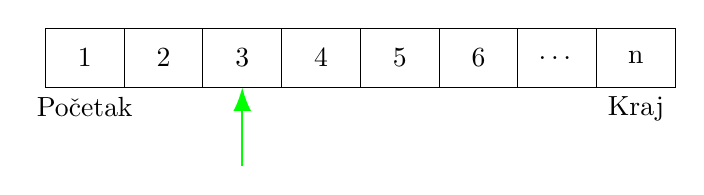
\begin{tikzpicture}[
  start chain=going right,
  node distance=0pt,
  box/.style={
    draw,
    minimum width=1cm,
    minimum height=0.75cm,
    on chain,
    inner sep=0pt,
    outer sep=0pt,
    text centered
  },
  arr/.style={
    -{Latex[length=3mm]},
    thick,
    green
  }
]

% Boxes
\node [box] (1) {1};
\node [box] (2) {2};
\node [box] (3) {3};
\node [box] (4) {4};
\node [box] (5) {5};
\node [box] (6) {6};
\node [box] (dots) {\dots};
\node [box] (n) {n};

% Labels aligned with boxes
\node [below=of 1.south, anchor=north] {Početak};
\node [below=of n.south, anchor=north] {Kraj};

% Arrow pointing to box 3 from below
\draw [arr] ([yshift=-1cm]3.south) -- (3.south);

\end{tikzpicture}
\end{center}
\end{frame}

\begin{frame}
    \frametitle{Direktno/nasumično}
    \begin{center}
        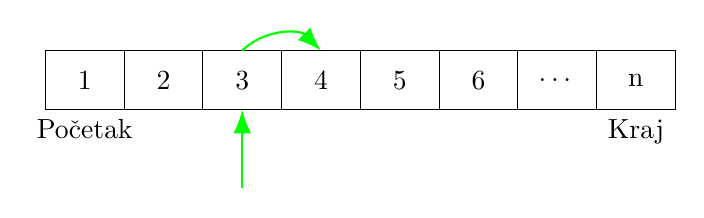
\begin{tikzpicture}[
            start chain=going right,
            node distance=0pt,
            box/.style={
                draw,
                minimum width=1cm,
                minimum height=0.75cm,
                on chain,
                inner sep=0pt,
                outer sep=0pt,
                text centered
  },
  arr/.style={
    -{Latex[length=3mm]},
    thick,
    green
  }
]

% Boxes
% (Same as previous slide)
% Boxes
\node [box] (1) {1};
\node [box] (2) {2};
\node [box] (3) {3};
\node [box] (4) {4};
\node [box] (5) {5};
\node [box] (6) {6};
\node [box] (dots) {\dots};
\node [box] (n) {n};

% Labels aligned with boxes
\node [below=of 1.south, anchor=north] {Početak};
\node [below=of n.south, anchor=north] {Kraj};

% Labels
% (Same as previous slide)

% Arrow pointing to box 3 from below
% (Same as previous slide)
\draw [arr] ([yshift=-1cm]3.south) -- (3.south);

% Arch arrow from 3 to 4
\draw [arr, bend left=45] (3.north) to (4.north);

\end{tikzpicture}
\end{center}
\end{frame}

\begin{frame}
    \frametitle{Direktno/nasumično}
\begin{center}
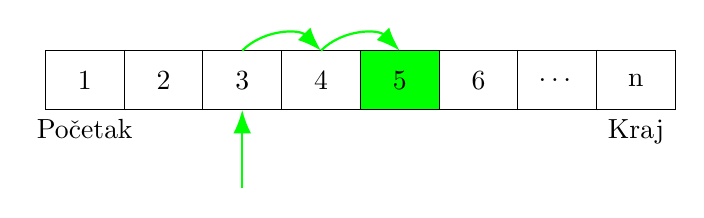
\begin{tikzpicture}[
  start chain=going right,
  node distance=0pt,
  box/.style={
    draw,
    minimum width=1cm,
    minimum height=0.75cm,
    on chain,
    inner sep=0pt,
    outer sep=0pt,
    text centered
  },
  arr/.style={
    -{Latex[length=3mm]},
    thick,
    green
  }
]

\node [box] (1) {1};
\node [box] (2) {2};
\node [box] (3) {3};
\node [box] (4) {4};
\node [box, fill=green!100] (5) {5};
\node [box] (6) {6};
\node [box] (dots) {\dots};
\node [box] (n) {n};

\node [below=of 1.south, anchor=north] {Početak};
\node [below=of n.south, anchor=north] {Kraj};

\draw [arr] ([yshift=-1cm]3.south) -- (3.south);

\draw [arr, bend left=45] (3.north) to (4.north);

\draw [arr, bend left=45] (4.north) to (5.north);

\end{tikzpicture}
\end{center}
\end{frame}


\begin{frame}
    \frametitle{Preko indeksa}
    \begin{itemize}
        \item Indeksni fajl (logički ključevi na fizičke adrese) \newline
        \item Brzina i efikasnost
    \end{itemize}
\end{frame}

\subsection*{}

\begin{frame}
    \frametitle{Alokacija memorije za fajl}
    \begin{itemize}
        \item Contigous Allocation \begin{itemize}
            \item Zauzeta memorija za fajl je kontinualna \newline
        \end{itemize}
        \item Linked Allocation \begin{itemize}
            \item Sadrži pokazivače na različite blokove diska \newline
        \end{itemize}
        \item Indexed Allocation \begin{itemize}
            \item Sadrži listu svih indeksa blokova fajla
        \end{itemize}
    \end{itemize}
\end{frame}

\begin{frame}
    \frametitle{Razvoj strukture direktorijuma}
    \begin{itemize}
        \item Jedan nivo \newline
        \item Dva nivoa (korisnik/direktorijum/fajl) \newline
        \item Stablo \newline
        \item Acikličan graf
    \end{itemize}
\end{frame}

\subsection*{Razvoj strukture direktorijuma}
\begin{frame}
    \frametitle{Jedan nivo}
    \begin{itemize}
        \item Višekorisnički operativni sistem \newline
        \item Svaki korisnik ima svoj dikretorijum 
    \end{itemize}
\end{frame}

\begin{frame}
    \frametitle{Dva nivoa}
    \begin{itemize}
        \item Kao za jedan nivo ali korisnik može da pravi direktorijume u tom nivou
    \end{itemize}

\end{frame}

\begin{frame}
    \frametitle{Stablo}
    \begin{itemize}
        \item Nema ograničenja na dubinu \newline
        \item Ne postoje linkovi
    \end{itemize}
\end{frame}

\begin{frame}
    \frametitle{Acikličan graf}
    \begin{itemize}
        \item Uvode se i linkovi
    \end{itemize}

\end{frame}

\subsection*{}

\begin{frame}
    \frametitle{Operacije nad sistemom fajlova}
    \begin{itemize}
        \item Otvaranje/zatvaranje fajlova \newline
        \item Dodavanje fajlova \newline
        \item Brisanje fajlova \newline
        \item Premeštanje fajlova
    \end{itemize}
\end{frame}

\begin{frame}
    \frametitle{Pouzdanost fajl sistema}
    \begin{itemize}
        \item Loši blokovi \newline
        \item Backup (sigurnosne kopije)
    \end{itemize}
\end{frame}

\begin{frame}
    \frametitle{RAID - \textit{Redundant Array of Independent Disks}}
    \begin{itemize}
        \item Pravljenje backup-a fajlova \newline
        \item RAID 0 \newline
        \item RAID 1 \newline
        \item RAID 5 \newline
        \item RAID 10 \newline
    \end{itemize}
\end{frame}

\subsection*{}
\section*{}

\begin{frame}
    \frametitle{Dokle smo stigli?}
    \begin{itemize}
        \item Pojam \newline
        \item Učitavanje operativnog sistema \newline
        \item Procesi \newline
        \item Planeri procesa \newline
        \item Zaštita memorije \newline
        \item Fajl sistemi
    \end{itemize}
\end{frame}

\begin{frame}
    \frametitle{Šta dalje?}
    \begin{itemize}
        \item Virtualizacija \newline
        \item Cloud \newline
        \item Distribuirani sistemi \newline
        \item Operativni sistemi koji se izvršavaju u realnom vremenu \newline
        \item Embedded sistemi \newline
        \item \dots
    \end{itemize}
\end{frame}

\begin{frame}
    \frametitle{HVALA NA PAŽNJI!}
    \begin{center}
        \Huge Pitanja?    
    \end{center}
\end{frame}

\end{document}